\documentclass{article}
\usepackage{ctex}
\usepackage[utf8]{inputenc}
\usepackage[hybrid]{markdown}
\usepackage[nottoc]{tocbibind}
\usepackage{changepage}
\usepackage{amsmath}
\usepackage{amssymb}
\usepackage{amsfonts}
\usepackage{amsthm}
\usepackage{enumerate}
\usepackage{authblk}
\usepackage{bm}
\newcommand*{\everymodeprime}{\ensuremath{\prime}}
%\usepackage{algorithm}
%\usepackage{algorithmic}
%\renewcommand{\algorithmicrequire}{ \textbf{Input:}} %Use Input in the format of Algorithm
%\renewcommand{\algorithmicensure}{ \textbf{Output:}} %UseOutput in the format of Algorithm
\usepackage[linesnumbered,lined,ruled,vlined,commentsnumbered]{algorithm2e}

\usepackage[colorlinks,linkcolor=blue,anchorcolor=blue,citecolor=blue,bookmarks = True]{hyperref}
\usepackage{longtable}
\usepackage{multirow}
\usepackage{float}
\usepackage{subfig}
\newcommand{\myI}{\mathbb{I}}
\newcommand{\mye}{\mathbb{E}}
\newcommand{\myd}{\mathrm{d}}
\newcommand{\pr}{\mathrm{Pr}}

\usepackage{bbm}
\newcommand{{\bmf}}{\bm{F}}
\newcommand{\bmd}{\bm{D}}
\newcommand{\bmx}{\bm{X}}
\newcommand{\bmr}{\bm{r}}
\newcommand{\myi}{\mathbbm{1}}

\newcommand{\etal}{\emph{et al.} }
\usepackage{booktabs}
\usepackage{graphics}
\usepackage{graphicx}
\usepackage[margin=25mm]{geometry}
\usepackage{color}

% \usepackage{abstract}
% \usepackage{autoref}
\newtheorem{theorem}{Theorem}[section]
\newtheorem{lemma}{Lemma}[section]
\def\lemmaautorefname{Lemma}
\newtheorem{definition}{Definition}[section]
\newtheorem{corollary}{Corollary}[section]
\def\corollaryautorefname{Corollary}
% \newtheorem{proposition}[theorem]{Proposition}
% \def\propositionautorefname{Proposition}
\newtheorem{remark}{Remark}
\renewcommand{\sectionautorefname}{Section}
\usepackage{graphicx}
\pagenumbering{gobble}
\usepackage{verbatim}
\usepackage{listings}
\usepackage{xcolor}

\definecolor{codegreen}{rgb}{0,0.6,0}
\definecolor{codegray}{rgb}{0.5,0.5,0.5}
\definecolor{codepurple}{rgb}{0.58,0,0.82}
\definecolor{backcolour}{rgb}{0.95,0.95,0.92}

\lstdefinestyle{mystyle}{
    backgroundcolor=\color{backcolour},   
    commentstyle=\color{codegreen},
    keywordstyle=\color{magenta},
    numberstyle=\tiny\color{codegray},
    stringstyle=\color{codepurple},
    basicstyle=\ttfamily\footnotesize,
    breakatwhitespace=false,         
    breaklines=true,                 
    captionpos=b,                    
    keepspaces=true,                 
    numbers=left,                    
    numbersep=5pt,                  
    showspaces=false,                
    showstringspaces=false,
    showtabs=false,                  
    tabsize=2
}

\lstset{style=mystyle}
% \usepackage{leftidx}
% correct bad hyphenation here
\title{\textbf{频繁项集挖掘算法-Apriori算法实现}}
\author{交叉研20 $\quad\quad$ 谭泽人 $\quad\quad$ 2020211335}
\date{\today}

\begin{document}
\maketitle

\section{引言}
关联规则是在给定数据项集上频繁出现的两个项集之间的关系。两个项集具有一定的关联规则需要具备两个条件,首先是他们都是频繁出现的,即他们的出现次数需要满足一个认为设定的参数,在本实验中为\texttt{minSup}。其次是,他们的出现需要具有一定的联系,在本实验中用confidence即置信度来衡量两个项集出现的关系。通过挖掘关联规则,我们可以找到两个项集之间出现之间的关系,通过关联规则我们可以通过一个项集的出现预测另一个项集出现的概率。它在现实生活中有需要应用,例如购物篮数据分析,网页预取,交叉购物,个性化网站,网络入侵检测。商家可以通过挖掘顾客购物的关联规则来设计商店的促销规则,从而获取更高的利润。例如在Walmart超市,通过对购物票据的挖掘,发现成年男性在购买啤酒的同时会同时购买尿不湿,超市通过将啤酒和尿不湿捆在一起做活动——购买尿不湿送啤酒,促进了更多人购买尿不湿,从而获得更高的盈利。因此关联规则挖掘在现实生活中十分重要。

关联规则挖掘首先被Agrawal \etal 提出 \cite{agrawal1993mining}。 在这之后有很多的算法被提出,例如Apriori算法 \cite{agarwal1994fast},FP-Growth \cite{han2000mining},CHARM算法 \cite{zaki2002charm},CLOSET+算法 \cite{wang2003closet+}等。 Apriori算法作为较为基础的算法,是学习关联股则挖掘算法的基础,因此本实验将实现该算法,并且评测其性能。

\section{算法概述}
在Apriori算法中,我们需要先指定一个度量一个项集的出现是否频繁的参数minimum support,出现次数大于minimum support的项集是频繁的。Apriori算法首先扫描一遍数据,找到只包含一个项并且频繁的项的集合。之后递归的生成包含$k$个项的频繁项集,直到没有更大的项集可以生成。在此过程中所生成的项集必须是频繁的,即出现的次数大于minimum support。Apriori算法的伪代码如下:
\begin{algorithm}[H]
\SetAlgoLined
\SetKwInOut{Input}{Input}\SetKwInOut{Output}{Output}
\caption{Apriori}
\BlankLine
$L_1\leftarrow$ the set of frequent items\;
\For{$k=1;L_k\neq \emptyset;k++$}{
	$C_{k+1}\leftarrow\emptyset$\;
	\For{$i,j \in L_k$}{
		\If{$|i\cup j| = k+1$}{
			$C_{k+1}\leftarrow C_{k+1}\cup \{i\cup j\}$\;
		}
	}
	\For{every transaction $t$ in database}{
		\For{$c\in C_{k+1}$}{
			\If{$c\subset t$}{
				the frequency of $c$ increases 1\;
			}
		}
	}
	\For{$c\in C_{k+1}$}{
		\If{frequency of $c\geq $minSup }{
			$L_{k+1}\leftarrow L_{k+1}\cup c$\;
		}
	}
}
return $\cup_k L_k$\;
\end{algorithm}

\section{算法实现}
\subsection{数据处理}
我使用的是老师提供的\texttt{groceries.csv}文件,其每一行包含一条交易数据,每条交易数据由一个交易的item数量和各个item组成:
\begin{figure}
\centering
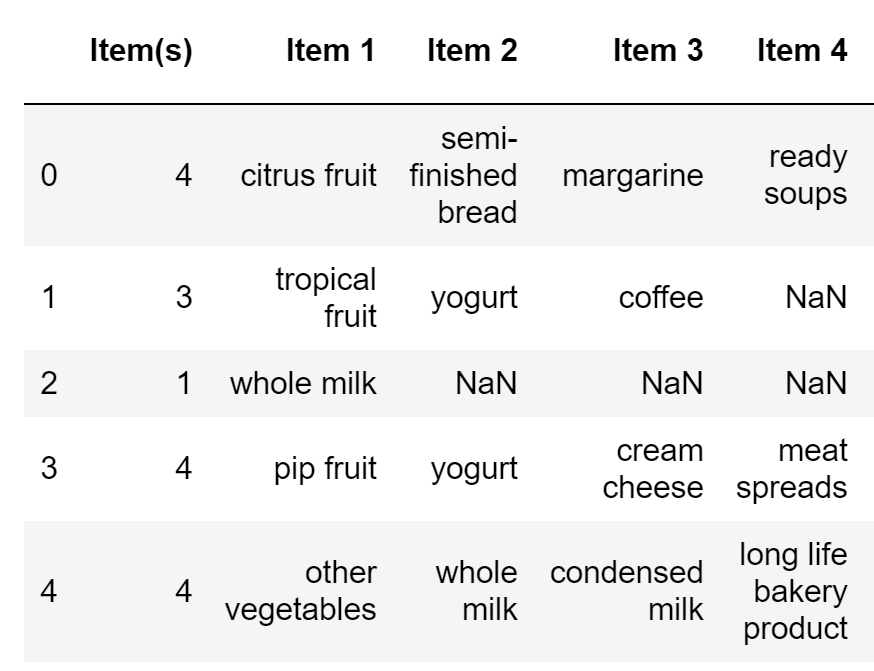
\includegraphics[width=10cm]{./pic/data}
\caption{数据样例}
\end{figure}

我先读取数据,利用python中的\texttt{set}数据类型保存数据,生成包含所有交易数据的一个Python generator:
\begin{lstlisting}[language=Python]
def readDataFromFile(filename):
    '''
    parameter(s)::
        filename: the file name that is going to be read. 
    return::
        a generator contains all transactions
    '''
    with open(filename,'r') as file:
        for line in file:
            line = line.rstrip(',\n')
            record = frozenset(line.split(',')[1:])
            yield record
\end{lstlisting}

并从中利用python set类型保存所有交易的item,用python list保存所有的交易:
\begin{lstlisting}[language = Python]
def getItemSetTransactionList(transactionGenerator):
    '''
    parameter(s)::
        transactionGenerator: a generator contains all transactions
    return::
        itemSet: the set of items exist in all transactions
        transactionList: a python list contains all transactions
    '''
    itemSet = set()
    transactionList = list()
    for record in transactionGenerator:
        transaction = frozenset(record)
        transactionList.append(transaction)
        for item in transaction:
            itemSet.add(frozenset([item]))
            
    return itemSet, transactionList

\end{lstlisting}

Apriori算法的主体如下:
\begin{lstlisting}[language=Python]
def Apriori(transactionGenerator, minSup, minConf):
    '''
    parameter(s)::
        transactionGenerator: a generator contains all transaction
        minSup: minimum support
        minConf: minimum confidence
    return::
        LSetDict: a dictionary consists of patterns of all length that satisfy the minimum support constraint
        freqPattern: a python list contains all frequent pattern
        associationRule: a python list contains all association rule satisfy minimum support and minimum confidence constraints
    '''
    itemSet, transactionList = getItemSetTransactionList(transactionGenerator)
    freqDict = defaultdict(int)
    LOneCandidate = minSupFilter(itemSet,transactionList,minSup,freqDict)
    k = 2
    LSetDict = dict()
    currentLSet = LOneCandidate
    while (currentLSet != set()):
        LSetDict[k-1] = currentLSet
        tempSet = currentLSet
        currentLSet = generateLkSet(tempSet,k)
        currentCSet = minSupFilter(currentLSet,transactionList,minSup,freqDict)
        currentLSet = currentCSet  
        k += 1

    freqPattern = list()
    for key, lset in LSetDict.items():
        freqPattern.extend([(set(item),freqDict[item]) for item in lset])
    associationRule = list()
    for key, lset in list(LSetDict.items())[1:]:
        for lseq in lset:
            properSubsets = [frozenset(x) for x in properSubset(lseq)]
            for item in properSubsets:
                if (len(lseq.difference(item))>0):
                    conf = freqDict[lseq]/freqDict[item]
                    if conf >= minConf:
                        associationRule.append([set(item),set(lseq.difference(item)),conf])
    return LSetDict, freqPattern,associationRule  
\end{lstlisting}

先生成只包含一个item的满足minSup要求的频繁项集\texttt{LOneCandidate},之后递归的生成包含$k$个item的频繁项集并保存在\texttt{LSetDict[k]}中。\texttt{freqPattern}包含所有的频繁项集及其相应的support。\texttt{associationRule}包含了所有的关联规则以及相应的confidence。

运行结果示例:
\begin{lstlisting}[language=Python]
>>> path = 'groceries.csv'
>>> file = readDataFromFile(path)
>>> minSup = 100
>>> minConf = 0.5
>>> t1 = datetime.now()
>>> LSetDict, freqPattern, associationRule = Apriori(file,minSup,minConf)
>>> t2 = datetime.now()
>>> print('Total running time of Apriori with minSup %d, minConf %.2f is: %.4f s' %(minSup,minConf,(t2-t1).seconds))
Total running time of Apriori with minSup 100, minConf 0.50 is: 5.0000 s
>>> freqPatternDF = pd.DataFrame(freqPattern)
>>> freqPatternDF.columns = ['pattern','frequency']
\end{lstlisting}
% 利用\texttt{pandas}展示的\texttt{freqPatternDF}的后面5行结果如下图所示。
% \begin{figure}
% \centering
% 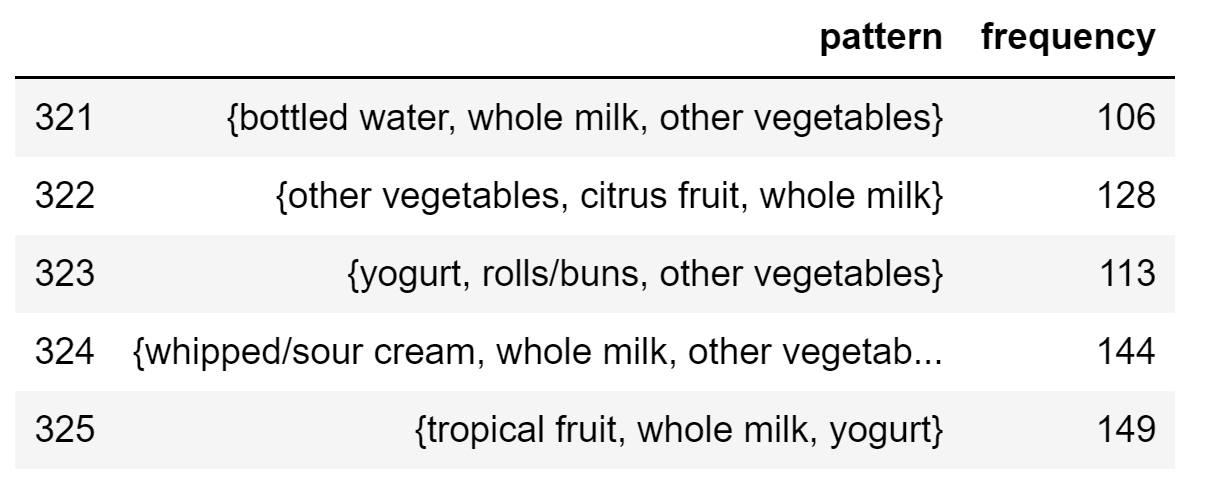
\includegraphics[width=10cm]{./pic/pattern}
% \caption{\texttt{freqPatternDF}的后面5行}
% \end{figure}

在设定\texttt{minSup}为100的情况下,求解出的包含一个元素的频繁项集有88个,包含两个元素的频繁项集有221个,包含三个元素的频繁项集有32个。其中出现频率最高的物品是“whole milk”,共在2513个订单中出现,其次为“other vegetables”,出现了1903次。出现频率较高的项集如表~\ref{tab:freq}~所示。
\begin{table}
\centering
\caption{出现频率最高的项集}
\label{tab:freq}
\begin{tabular}{c|c||p{5.5cm}|c||p{5.5cm}|c}
\hline 
项集 & 频率 & 项集 & 频率 & 项集 & 频率\\
\hline\hline
whole milk & 2513 & whole milk, other vegetables&736 &root vegetables, whole milk, other vegetables & 228\\
\hline 
other vegetables & 1903 & rolls/buns, whole milk & 557 & yogurt, whole milk, other vegetables&219 \\
\hline 
rolls/buns & 1809 & whole milk, yogurt & 551 &yogurt, rolls/buns, whole milk & 153\\
\hline 
soda & 1715 & whole milk, root vegetables & 481 &tropical fruit, whole milk, yogurt & 149\\
\hline 
yogurt & 1372 & root vegetables, other vegetables & 466 & whipped/sour cream, whole milk, other vegetables&144 \\
\hline 
\end{tabular}
\end{table}

confidence 不小于0.5的关联规则共有15个,分别如表~\ref{tab:assorules}~所示:
\begin{table}
\centering
\caption{confidence大于0.5的关联规则}
\label{tab:assorules}
\begin{tabular}{ccc}
\hline 
X & Y & confidence\\
\hline\hline
yogurt, root vegetables &  other vegetables & 0.500\\
rolls/buns, root vegetables &  other vegetables & 0.502\\
whipped/sour cream, other vegetables& whole milk &    0.507\\
other vegetables, yogurt & whole milk  &  0.513\\
tropical fruit, yogurt & whole milk & 0.517\\
pip fruit, other vegetables & whole milk & 0.518\\
rolls/buns, root vegetables & whole milk &  0.523\\
whipped/sour cream, yogurt & whole milk & 0.525\\
other vegetables, domestic eggs & whole milk & 0.553\\
yogurt, root vegetables & whole milk & 0.563\\
tropical fruit, root vegetables & whole milk & 0.570\\
other vegetables, butter & whole milk&  0.574\\
curd, yogurt & whole milk & 0.582\\
tropical fruit, root vegetables & other vegetables& 0.585\\
citrus fruit, root vegetables & other vegetables &  0.586\\
\hline 
\end{tabular}
\end{table}
% \begin{figure}
% \centering
% 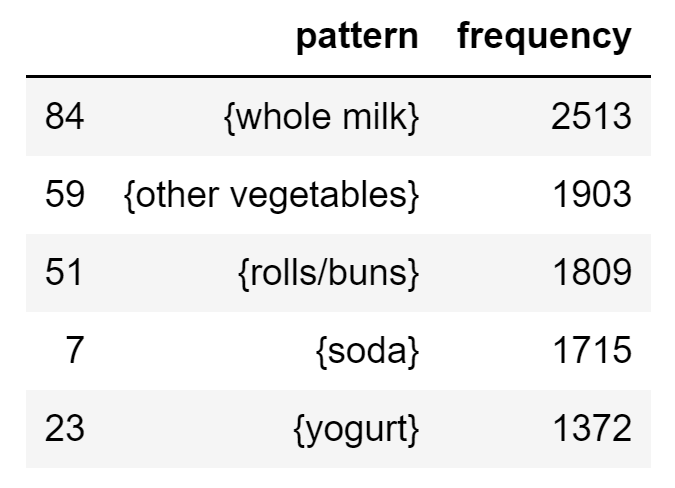
\includegraphics[width=10cm]{./pic/freqpatternone}
% \caption{出现频率前五的物品}
% \end{figure}

\section{不同参数下算法的结果}
我的算法中设置了两个参数minSup和minConf,分别代表support的最小阈值和confidence的最小阈值。我在不同的参数设定下分别运行算法。实验环境为windows 10环境下laptop CPU@1.60GHz。 
\subsection{不同minSup下的结果}
随着minSup的增大,将会有更多的项集因为出现的次数不够多而被剪枝,从而最终得到的频繁项集的大小以及关联规则的大小都将减小,如图~\ref{fig:minsup}~所示。
\begin{figure}
\centering
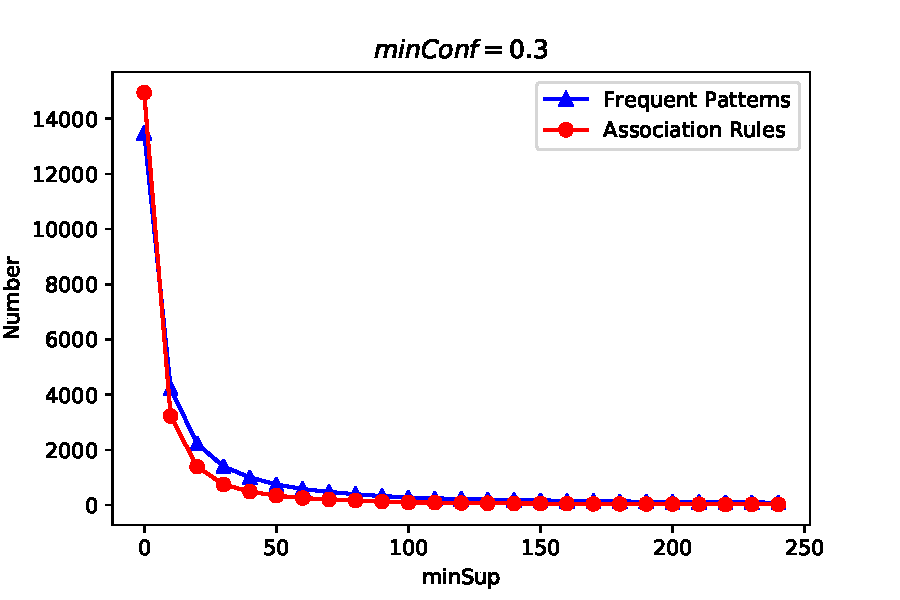
\includegraphics[width=7cm]{./pic/minsup}
\caption{不同minSup下的结果}
\label{fig:minsup}
\end{figure}

并且因为剪枝增加,算法运行时间减小。
\begin{figure}
\centering
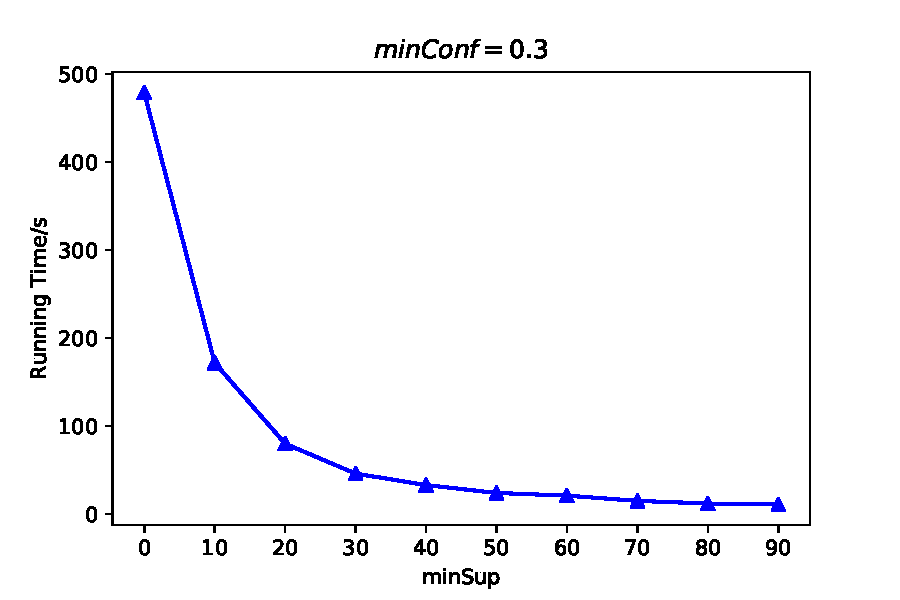
\includegraphics[width=10cm]{./pic/timesup}
\caption{不同minSup下的算法运行时间}
\label{fig:time}
\end{figure}

\subsection{不同minConf下的结果}
minConf只影响关联规则的挖掘,随着minConf增大,关联规则被剪枝越多,最终满足约束的关联规则数量减少,但是频繁项集的数量不受影响,如图~\ref{fig:minconf}~所示。
\begin{figure}
\centering
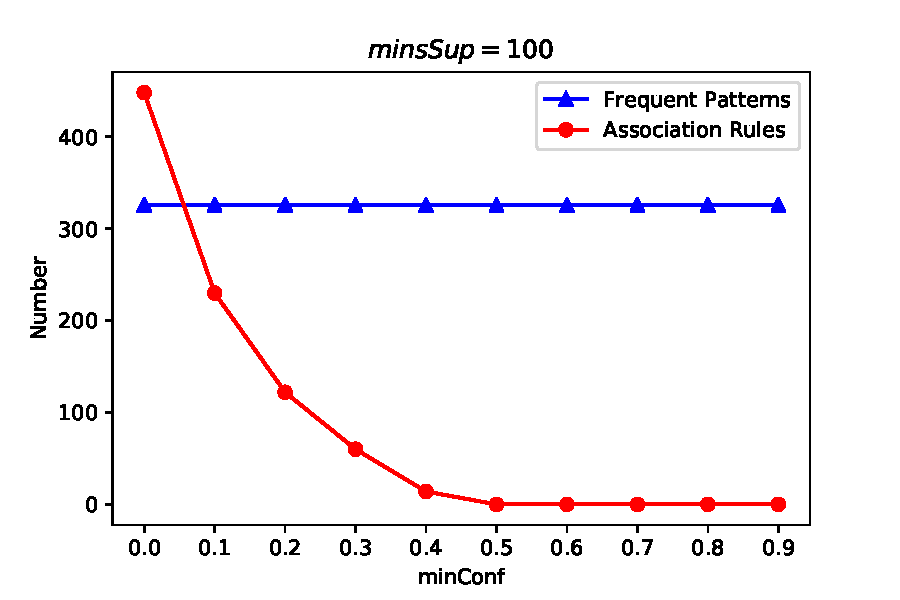
\includegraphics[width=10cm]{./pic/minconf}
\caption{不同minConf下的结果}
\label{fig:minconf}
\end{figure}


\section{实验代码}
所有代码都在\href{https://github.com/thutzr/DataMining2020Autumn}{这里}。提交的结果中包含一个\texttt{Apriori.py}和一个\texttt{Apriori.ipynb}文件,ipynb文件中包含了算法的实现和实验的结果,比较详细,可读性铰.py文件更强。如果需要运行.py文件,请在命令行输入以下命令:
\begin{lstlisting}[language=command.com]
$ python -f file.csv -s minSup -c minConf -of freqPath -oa assoPath
\end{lstlisting}
其中,\texttt{-f}用于指定csv文件,\texttt{-s}用于指定minSup,\texttt{-c}用于指定minConf,\texttt{-of}和\texttt{-oa}分别用于指定freqPatterns和associationRules存储的路径。默认的minSup为10,默认的minConf为0.3,freqPath和assoPath分别默认为freqPattern.csv和associationRules.csv。
\bibliographystyle{plain}
\bibliography{ref.bib}
\end{document}